% Intended LaTeX compiler: pdflatex
\documentclass[10pt,a4paper,UTF8]{article}
\usepackage{zclorg}
\usepackage{tikztheorem}
\author{zcl.space}
\date{}
\title{随机变量函数的分布}
\hypersetup{
 pdfauthor={zcl.space},
 pdftitle={随机变量函数的分布},
 pdfkeywords={probability},
 pdfsubject={},
 pdfcreator={Emacs 25.0.50.1 (Org mode 9.0.6)},
 pdflang={English}}
\begin{document}

\maketitle
\tableofcontents
\titlepic{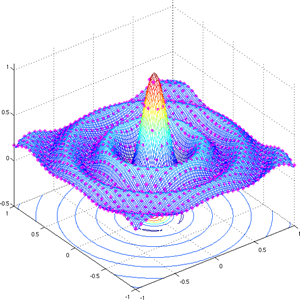
\includegraphics[scale=0.25]{../../img/sinc.PNG}}

\section{引子}
\label{sec:orgf24f4ed}


我们经常遇到这样的情形:已知某个随机变量的分布,但我们感兴趣的是该随机变量的函数的分布。例如,设随机变量\(X\)的分布已知,欲求\(g(X)\)的分布。为求\(g(X)\)的分布,需要将事件\(g(X) \leq y\)表示关于\(X\)的集合。
\section{几个例子}
\label{sec:orgcaa50a1}


\begin{tikzinstance}
设随机变量\(X\)服从\((0,1)\)上的均匀分布,下面我们给出随机变量\(Y = X^{n}\)的分布。对于\(0 \leq y \leq 1\)有:
\begin{eqnarray}
\label{eq:1}
F_{Y}(y) &=& P\{Y \leq y\}  \\
&=& P\{X^{n} \leq y\} \\
&=& P\{X \leq y^{1/n}\} \\
&=& F_{X}(y^{1/n}) \\
&=& y^{1/n}
\end{eqnarray}
则\(Y\)的密度函数为:
\begin{equation}
\label{eq:2}
f_{Y}(y) =
\begin{cases}
\frac{1}{n}y^{\tfrac{1}{n}-1} & 0 \leq y \leq 1 \\
0 & \mathrm{others}
\end{cases}
\end{equation}
\end{tikzinstance}

\begin{tikzinstance}
设\(X\)是一个连续性随机变量,密度函数为\(f_{X}\),则\(Y = X^{2}\)的分布可以通过以下方法得到:对于\(y\geq 0\),有:
\begin{equation}
\label{eq:3}
F_{Y}(y) = P\{Y\leq y\} = P\{X^{2} \leq y\}  = P\{-\sqrt{y} \leq X \leq \sqrt{y} \} = F_{X}(\sqrt{y}) - F_{x}(-\sqrt{y})
\end{equation}
求导可得:
\begin{equation}
\label{eq:4}
f^{Y}(y) = \frac{1}{2\sqrt{y}} [f_{X}(\sqrt{y}) + f_{X}(-\sqrt{y}) ]
\end{equation}
\end{tikzinstance}

\begin{tikzinstance}
设\(X\)有密度函数\(f_{X}\),则\(Y=|X|\)的密度函数可以如下得到,对于\(y\geq 0\),有:
\begin{equation}
\label{eq:5}
F_{Y}(y) = P\{Y \leq y\} = P\{ |X| \leq y\} = P\{ -y \leq X \leq y\} = F_{X}(y) - F_{X}(-y)
\end{equation}
求导可得:
\begin{equation}
\label{eq:6}
f_{Y}(y) = f_{X}(y) + f_{X}(-y) ,y\geq 0
\end{equation}
\end{tikzinstance}
\section{一般性的定理}
\label{sec:orgfbd4c25}


\begin{tikztheorem}
设\(X\)为连续随机变量,密度函数为\(f_{X}\),设\(g(x)\)为一严格单调(递增或递减)且可微的函数,那么随机变量\(Y=g(X)\)的密度函数为:
\begin{equation}
\label{eq:7}
f_{Y}(y) =
\begin{cases}
f_{X}[g^{-1}(y)]|\frac{\mathrm{d}}{\mathrm{d}y}g^{-1}(y)| & \mathrm{if}\exists x,s.t. y = g(x)\\
0 & \forall x, y\neq g(x)
\end{cases}
\end{equation}
\end{tikztheorem}
\begin{tikzproof}
设对某些\(x\),有\(y=g(x)\),那么,若令\(Y = g(X)\),则有:
\begin{equation}
\label{eq:9}
F_{Y}(y) = P\{g(X)\leq y\} = P\{X \leq g^{-1}(y)\} = F_{X}(g^{-1}(y))
\end{equation}
求导可得:
\begin{equation}
\label{eq:10}
f_{Y}(y) = f_{X}(g^{-1}(y)) \frac{\mathrm{d}}{\mathrm{d}y}g^{-1}(y)
\end{equation}
因为\(g^{-1}(y)\)单调非降,所以导数非负。若\(g^{-1}(y)\)单调非曾则导数为负值。

若对于任意\(x\)都有\(y\neq g(x)\),那么\(F_{Y}(y)\)要么是0要么是1.无论哪种情况都有\(f_{Y}(y) = 0\)
\end{tikzproof}
\end{document}
